\documentclass[12pt]{article}
\usepackage{lecture}
\usepackage{graphics}
\usepackage{html}
\usepackage{url}

\newcommand{\copyrightYears}{2001-2015}

\title{Patterns of nucleotide and amino acid substitution}

\begin{document}

\maketitle

\thispagestyle{first}

\section*{Introduction}

So I've just suggested that the neutral theory of molecular evolution
explains quite a bit, but it also ignores quite a bit.\footnote{I
  won't make my bikini joke, because it doesn't conceal as much as
  quantitative gentics. But still the ``pure'' version of the neutral
  theory of molecular evolution makes a {\it lot\/} of simplifying
  assumptions.} The derivations we did assumed that all substitutions
are equally likely to occur, because they are selectively
neutral. That isn't plausible. We need look no further than sickle
cell anemia to see an example of a protein polymorphism in which a
single amino acid difference has a very large effect on fitness. Even
reasoning from first principles we can see that it doesn't make much
sense to think that all nucleotide substitutions are created
equal. Just as it's unlikely that you'll improve the performance of
your car if you pick up a sledgehammer, open its hood, close your
eyes, and hit something inside, so it's unlikely that picking a random
amino acid in a protein and substituting it with a different one will
improve the function of the protein.\footnote{Obviously it happens
  sometimes. If it didn't, there wouldn't be any adaptive
  evolution. It's just that, on average, mutations are more likely to
  decrease fitness than to increase it. }\index{sledgehammer principle}

\section*{The genetic code}

Of course, not all nucleotide sequence substitutions lead to amino
acid substitutions in protein-coding genes. There is redundancy in the
genetic code. Table~\ref{table:code} is a list of the codons in the
universal genetic code.\footnote{By the way, the ``universal'' genetic
  code is not universal. There are at least eight, but all of them
  have similar redundancy properties.} Notice that there are only two
amino acids, methionine and tryptophan, that have a single codon. All the
rest have at least two. Serine, arginine, and leucine have
six.\index{genetic code}

\begin{table}
\begin{center}
\begin{tabular}{llllllll}
\hline\hline
      & Amino &       & Amino &       & Amino &       & Amino \\
Codon & Acid  & Codon & Acid  & Codon & Acid  & Codon & Acid \\
\hline
UUU   & Phe   & UCU   & Ser   & UAU   & Tyr   & UGU   & Cys \\
UUC   & Phe   & UCC   & Ser   & UAC   & Tyr   & UGC   & Cys \\
UUA   & Leu   & UCA   & Ser   & UAA   & Stop  & UGA   & Stop \\
UUG   & Leu   & UCG   & Ser   & UAG   & Stop  & UGG   & Trp \\
      &       &       &       &       &       &       & \\
CUU   & Leu   & CCU   & Pro   & CAU   & His   & CGU   & Arg \\
CUC   & Leu   & CCC   & Pro   & CAC   & His   & CGC   & Arg \\
CUA   & Leu   & CCA   & Pro   & CAA   & Gln   & CGA   & Arg \\
CUG   & Leu   & CCG   & Pro   & CAG   & Gln   & CGG   & Arg \\
      &       &       &       &       &       &       & \\
AUU   & Ile   & ACU   & Thr   & AAU   & Asn   & AGU   & Ser \\
AUC   & Ile   & ACC   & Thr   & AAC   & Asn   & AGC   & Ser \\
AUA   & Ile   & ACA   & Thr   & AAA   & Lys   & AGA   & Arg \\
AUG   & Met   & ACG   & Thr   & AAG   & Lys   & AGG   & Arg \\
      &       &       &       &       &       &       & \\
GUU   & Val   & GCU   & Ala   & GAU   & Asp   & GGU   & Gly \\
GUC   & Val   & GCC   & Ala   & GAC   & Asp   & GGC   & Gly \\
GUA   & Val   & GCA   & Ala   & GAA   & Glu   & GGA   & Gly \\
GUG   & Val   & GCG   & Ala   & GAG   & Glu   & GGG   & Gly \\
\hline
\end{tabular}
\end{center}
\caption{The universal genetic code.}\label{table:code}
\end{table}

Moreover, most of the redundancy is in the third position, where we
can distinguish 2-fold from 4-fold redundant
sites~(Table~\ref{table:fold}). 2-fold redundant sites are those at
which either one of two nucleotides can be present in a codon for a
single amino acid. 4-fold redundant sites are those at which any of
the four nucleotides can be present in a codon for a single amino
acid. In some cases there is redundancy in the first codon position,
e.g, both AGA and CGA are codons for arginine. Thus, many nucleotide
substitutions at third positions do not lead to amino acid
substitutions, and some nucleotide substitutions at first positions do
not lead to amino acid substitutions. But every nucleotide
substitution at a second codon position leads to an amino acid
substitution. Nucleotide substitutions that do not lead to amino acid
substitutions are referred to as {\it synonymous substitutions},
because the codons involved are synonymous, i.e., code for the same
amino acid. Nucleotide substitutions that do lead to amino acid
substituions are {\it non-synonymous substitutions}.\index{genetic code!redundancy}\index{synonymous substitutions}\index{non-synonymous substitutions} 

\begin{table}
\begin{center}
\begin{tabular}{lll}
\hline\hline
      & Amino & \\
Codon & Acid  & Redundancy \\
\hline
CCU   & Pro   & 4-fold \\
CCC \\
CCA \\
CCG \\
\hline
AAU   & Asn   & 2-fold \\
AAC \\
AAA   & Lys   & 2-fold \\
AAG \\
\hline
\end{tabular}
\end{center}
\caption{Examples of 4-fold and 2-fold redundancy in the 3rd position
  of the universal genetic code.}\label{table:fold}
\end{table}

\section*{Rates of synonymous and non-synonymous substitution}

By using a modification of the simple Jukes-Cantor model we
encountered before, it is possible make separate estimates of the
number of synonymous substitutions and of the number of non-synonymous
substitutions that have occurred since two sequences diverged from a
common ancestor. If we combine an estimate of the {\it number\/} of
differences with an estimate of the {\it time of divergence\/} we can
estimate the rates of synonymous and non-synonymous
substitution~(number/time). Table~\ref{table:substitution-data} shows some
representative estimates for the rates of synonymous and
non-synonymous substitution in different genes studied in
mammals.\index{substitution rates}

\begin{table}
\begin{center}
\begin{tabular}{lcc}
\hline\hline
Locus     & Non-synonymous rate & Synonymous rate \\
\hline
Histone \\
\quad H4  & 0.00                & 3.94 \\
\quad H2  & 0.00                & 4.52 \\ 
Ribosomal proteins \\
\quad S17 & 0.06                & 2.69 \\
\quad S14 & 0.02                & 2.16 \\
Hemoglobins \& myoglobin \\
\quad $\alpha$-globin & 0.56    & 4.38 \\
\quad $\beta$-globin  & 0.78    & 2.58 \\
\quad Myoglobin       & 0.57    & 4.10 \\
Interferons \\
\quad $\gamma$  & 3.06          & 5.50 \\
\quad $\alpha$1 & 1.47          & 3.24 \\
\quad $\beta$1  & 2.38          & 5.33 \\
\hline
\end{tabular}
\end{center}
\caption{Representative rates of synonymous and non-synonymous
  substitution in mammalian genes~(from~\cite{Li97}). Rates are
  expressed as the number of substitutions per $10^9$
  years.}\label{table:substitution-data}
\end{table}

Two very important observations emerge after you've looked at this
table for awhile. The first won't come as any shock. The rate of
non-synonymous substitution is generally lower than the rate of
synonymous substitution. This is a result of my ``sledgehammer
principle.'' Mutations that change the amino acid sequence of a
protein are more likely to reduce that protein's functionality than to
increase it. As a result, they are likely to lower the fitness of
individuals carrying them, and they will have a lower probability of
being fixed than those mutations that do not change the amino acid
sequence.\index{sledgehammer principle}

The second observation is more subtle. Rates of non-synonymous
substitution vary by more than two orders of magnitude: 0.02
substitutions per nucleotide per billion years in ribosomal protein
S14 to 3.06 substitutions per nucleotide per billion years in
$\gamma$-interferon, while rates of synonymous substitution vary only
by a factor of two (2.16 in ribosomal protein S14 to 4.52 in histone
H2). If synonymous substitutions are neutral, as they probably are to
a first approximation,\footnote{We'll see that they may not be
  completely neutral a little later, but at least it's reasonable to
  believe that the intensity of selection to which they are subject is
  less than that to which non-synonymous substitutions are subject.}
then the rate of synonymous substitution should equal the mutation
rate. Thus, the rate of synonymous substitution should be
approximately the same at every locus, which is roughly what we
observe. But proteins differ in the degree to which their
physiological function affects the performance and fitness of the
organisms that carry them. Some, like histones and ribosomal proteins,
are intimately involved with chromatin or translation of messenger RNA
into protein. It's easy to imagine that just about any change in the
amino acid sequence of such proteins will have a detrimental effect on
its function. Others, like interferons, are involved in responses to
viral or bacterial pathogens. It's easy to imagine not only that the
selection on these proteins might be less intense, but that some amino
acid substitutions might actually be favored by natural selection
because they enhance resistance to certain strains of pathogens. Thus,
the probability that a non-synonymous substitution will be fixed is
likely to vary substantially among genes, just as we observe.

\section*{Revising the neutral theory}

So we've now produced empirical evidence that many mutations are {\it
  not\/} neutral. Does this mean that we throw the neutral theory of
molecular evolution away? Hardly. We need only modify it a little to
accomodate these new observations.\index{neutral theory!modifications}

\begin{itemize}

\item {\it Most non-synonymous substitutions are deleterious.\/} We
  can actually generalize this assertion a bit and say that most
  mutations that affect function are deleterious. After all, organisms
  have been evolving for about 3.5 billion years. Wouldn't you expect
  their cellular machinery to work pretty well by now?

\item {\it Most molecular variability found in natural populations is
    selectively neutral.} If most function-altering mutations are
  deleterious, it follows that we are unlikely to find much variation
  in populations for such mutations. Selection will quickly eliminate
  them.

\item {\it Natural selection is primarily purifying.} Although natural
  selection for variants that improve function is ultimately the
  source of adaptation, even at the molecular level, most of the time
  selection is simply eliminating variants that are less fit than the
  norm, not promoting the fixation of new variants that increase
  fitness.

\item {\it Alleles enhancing fitness are rapidly incorporated.} They
  do not remain polymorphic for long, so we aren't likely to find
  them when they're polymorphic.

\end{itemize}

As we'll see, even these revisions aren't entirely sufficient, but
what we do from here on out is more to provide refinements and
clarifications than to undertake wholesale revisions.

\section*{Detecting selection on nucleotide polymorphisms}

At this point, we've refined the neutral theory quite a bit. Our
understanding of how molecules evolve now recognizes that some
substitutions are more likely than others, but we're still proceeding
under the assumption that most nucleotide substitutions are neutral or
detrimental. So far we've argued that variation like what Hubby and
Lewontin~\cite{Hubby-Lewontin66,Lewontin-Hubby66} found is not likely
to be maintained by natural selection. But we have strong evidence
that heterozygotes for the sickle-cell allele are more fit than either
homozygote in human populations where malaria is prevalent. That's an
example where selection is acting to maintain a polymorphism, not to
eliminate it. Are there other examples? How could we detect them?

In the 1970s a variety of studies suggested that a polymorphism in the
locus coding for alcohol dehydrogenase in {\it Drosophila
  melanogaster\/} might not only be subject to selection but that
selection may be acting to maintain the polymorphism. As DNA
sequencing became more practical at about the same time,\footnote{It
  was still {\it vastly\/} more laborious than it is now.} population
geneticists began to realize that comparative analyses of DNA
sequences at protein-coding loci could provide a powerful tool for
unraveling the action of natural selection. Synonymous sites within a
protein-coding sequence provide a powerful standard of
comparision. Regardless of

\begin{itemize}

\item the demographic history of the population from which the
  sequences were collected,

\item the length of time that populations have been evolving under the
  sample conditions and whether it has been long enough for the
  population to have reached a drift-migration-mutation-selection
  equilibrium, or

\item the actual magnitude of the mutation rate, the migration rate,
  or the selection coefficients

\end{itemize}

\noindent the synonymous positions within the sequence provide an
internal control on the amount and pattern of differentiation that
should be expected when substitutions.\footnote{Ignoring, for the
  moment, the possibility that there may be selection on codon usage.}
Thus, if we see different patterns of nucleotide substitution at
synonymous and non-synonymous sites, we can infer that selection is
having an effect on amino acid substitutions.

\subsection*{Nucleotide sequence variation at the {\it Adh\/} locus in
  {\it Drosophila melanogaster}}\index{Drosophila@\textit{Drosophila}!\textit{melanogaster}}\index{alcohol dehydrogenase}\index{Adh}

Kreitman~\cite{Kreitman83} took advantage of these ideas to provide
additional insight into whether natural selection was likely to be
involved in maintaining the polymorphism at {\it Adh\/} in {\it
  Drosophila melanogaster}. He cloned and sequenced 11 alleles at this
locus, each a little less than 2.4kb in length.\footnote{Think about
  how the technology has changed since then. This work represented a
  major part of his Ph.D. dissertation, and the results were published
  as an article in {\it Nature}.} If we restrict our attention to the
coding region, a total of 765bp, there were 6 distinct sequences that
differed from one another at between 1 and 13 sites. Given the
observed level of polymorphism within the gene, there should be 9 or
10 amino acid differences observed as well, but only one of the
nucleotide differences results in an amino acid difference, the amino
acid difference associated with the already recognized electrophoretic
polymorphsim. Thus, there is significantly less amino acid diversity
than expected if nucleotide substitutions were neutral, consistent
with my assertion that most mutations are deleterious and that natural
selection will tend to eliminate them.\index{Adh!purifying selection}
In other words, another example of the ``sledgehammer
principle.''\index{sledgehammer principle}

Does this settle the question? Is the {\it Adh\/} polymorphism another
example of allelic variants being neutral or selected against? Would I
be asking these questions if the answer were ``Yes''?

\subsubsection*{Kreitman and Aguad{\'e}}

A few years after Kreitman~\cite{Kreitman83} appeared, Kreitman and
Aguad{\'e}~\cite{Kreitman-Aguade86} published an analysis in which
they looked at levels of nucleotide diversity in the {\it Adh\/}
region, as revealed through analysis of RFLPs, in {\it
  D. melanogaster\/} and the closely related {\it D. simulans}. Why
the comparative approach? Well, Kreitman and Aguad{\'e} recognized
that the neutral theory of molecular evolution makes two predictions
that are related to the underlying mutation rate:

\begin{itemize}

\item If mutations are neutral, the substitution rate is equal to the
  mutation rate.

\item If mutations are neutral, the diversity within populations
  should be about $4N_e\mu/(4N_e\mu + 1)$.

\end{itemize}

\noindent Thus, if variation at the {\it Adh\/} locus in {\it
  D. melanogaster\/} is selectively neutral, the amount of divergence
between {\it D. melanogaster\/} and {\it D. simulans\/} should be
related to the amount of diversity within each. What they found
instead is summarized in Table~\ref{table:ka}.\index{Adh!balancing selection}\index{diversity-divergence}

\begin{table}
\begin{center}
\begin{tabular}{l|ccc}
\hline\hline
         & 5' flanking & {\it Adh\/} locus & 3' flanking \\
\hline
Diversity$^1$ \\
\quad Observed & 9     & {\bf 14}   & 2    \\
\quad Expected & 10.8  & 10.8 & 3.4  \\
Divergence$^2$ \\
\quad Observed & 86    & 48   & 31   \\
\quad Expected & 55    & {\bf 76.9} & 33.1 \\
\hline
\multicolumn{4}{l}{$^1$Number of polymorphic sites within {\it
         D. melanogaster\/}} \\
\multicolumn{4}{l}{$^2$Number of nucleotide differences between {\it
         D. melanogaster\/} and {\it D. simulans}}
\end{tabular}
\end{center}
\caption{Diversity and divergence in the {\it Adh\/} region of {\it
    Drosophila}~(from~\cite{Kreitman-Aguade86}).}\label{table:ka}
\end{table}

Notice that there is substantially less divergence at the {\it Adh\/}
locus than would be expected, based on the average level of divergence
across the entire region. That's consistent with the earlier
observation that most amino acid substitutions are selected
against. On the other hand, there is {\it more\/} nucleotide diversity
within {\it D. melanogaster\/} than would be expected based on the
levels of diversity seen in across the entire region. What gives?

Time for a trip down memory lane. Remember something called
``coalescent theory?'' It told us that for a sample of neutral genes
from a population, the expected time back to a common ancestor for all
of them is about $4N_e$ for a nuclear gene in a diploid
population. That means there's been about $4N_e$ generations for
mutations to occur. Suppose, however, that the electrophoretic
polymorphism were being maintained by natural selection. Then we might
well expect that it would be maintained for a lot longer than $4N_e$
generations. If so, there would be a lot more time for diversity to
accumulate. Thus, the excess diversity could be accounted for if there
is balancing selection at ADH.\index{coalescent!balancing selection}

\subsubsection*{Kreitman and Hudson}

Kreitman and Hudson~\cite{Kreitman-Hudson91} extended this approach by
looking more carefully within the region to see where they could find
differences between observed and expected levels of nucleotide
sequence diversity. They used a ``sliding window'' of 100 silent base
pairs in their calculations. By ``sliding window'' what they mean is
that first they calculate statistics for bases 1-100, then for bases
2-101, then for bases 3-102, and so on until they hit the end of the
sequence. It's rather like walking a chromosome for QTL mapping, and
the results are rather pretty~(Figure~\ref{fig:kh}). 

\begin{figure}
\begin{center}
\resizebox{!}{6cm}{\includegraphics{kreitman-hudson.eps}}
\end{center}
\caption{Sliding window analysis of nucleotide diversity in the {\it
    Adh\/}-{\it Adh-dup} region of {\it Drosophila melanogaster}. The
  arrow marks the position of the single nucleotide substitution that
  distinguishes {\it Adh-F\/} from {\it
    Adh-S\/}~(from~\cite{Kreitman-Hudson91})}\label{fig:kh}
\end{figure}

To me there are two particularly striking things about this
figure. First, the position of the single nucleotide substitution
responsible for the electrophoretic polymorphism is clearly
evident. Second, the excess of polymorphism extends for only a 200-300
nucleotides in each direction. That means that the rate of
recombination {\it within\/} the gene is high enough to randomize the
nucleotide sequence variation farther away.\footnote{Think about what
  that means for association mapping. In organisms with a large
  effective population size, associations due to physical linkage may
  fall off {\it very\/} rapidly, meaning that you would have to have a
  {\it very\/} dense map to have a hope of finding associations.}

\section*{Detecting selection in the human genome}

I've already mentioned the HapMap project~\cite{HapMap-2007}, a
collection of genotype data at roughly 3.2M SNPs in the human
genome. The data in phase II of the project were collected from four
populations:

\begin{itemize}

\item Yoruba (Ibadan, Nigeria)

\item Japanese (Tokyo, Japan)

\item Han Chinese (Beijing, China)

\item ancestry from northern and western Europe (Utah, USA)

\end{itemize}

We expect genetic drift to result in allele frequency differences
among populations, and we can summarize the extent of that
differentiation at each locus with $F_{ST}$. If all HapMap SNPs are
selectively neutral,\footnote{And unlinked to sites that are under
  selection.} then all loci should have the same $F_{ST}$ within the
bounds of statistical sampling error and the evolutionary sampling due
to genetic drift. A scan of human chromosome 7 reveals both a lot of
variation in individual-locus estimates of $F_{ST}$ and a number of
loci where there is substantially more differentiation among
populations than is expected by
chance~(Figure~\ref{fig:low-res-SNP}). At very fine genomic scales we
can detect even more outliers~(Figure~\ref{fig:high-res-SNP}),
suggesting that human populations have been subject to divergent
selection pressures at many different loci~\cite{Guo-etal-2009}.\index{F-statistics@$F$-statistics!outliers}

\begin{figure}
\begin{center}
\resizebox{\textwidth}{!}{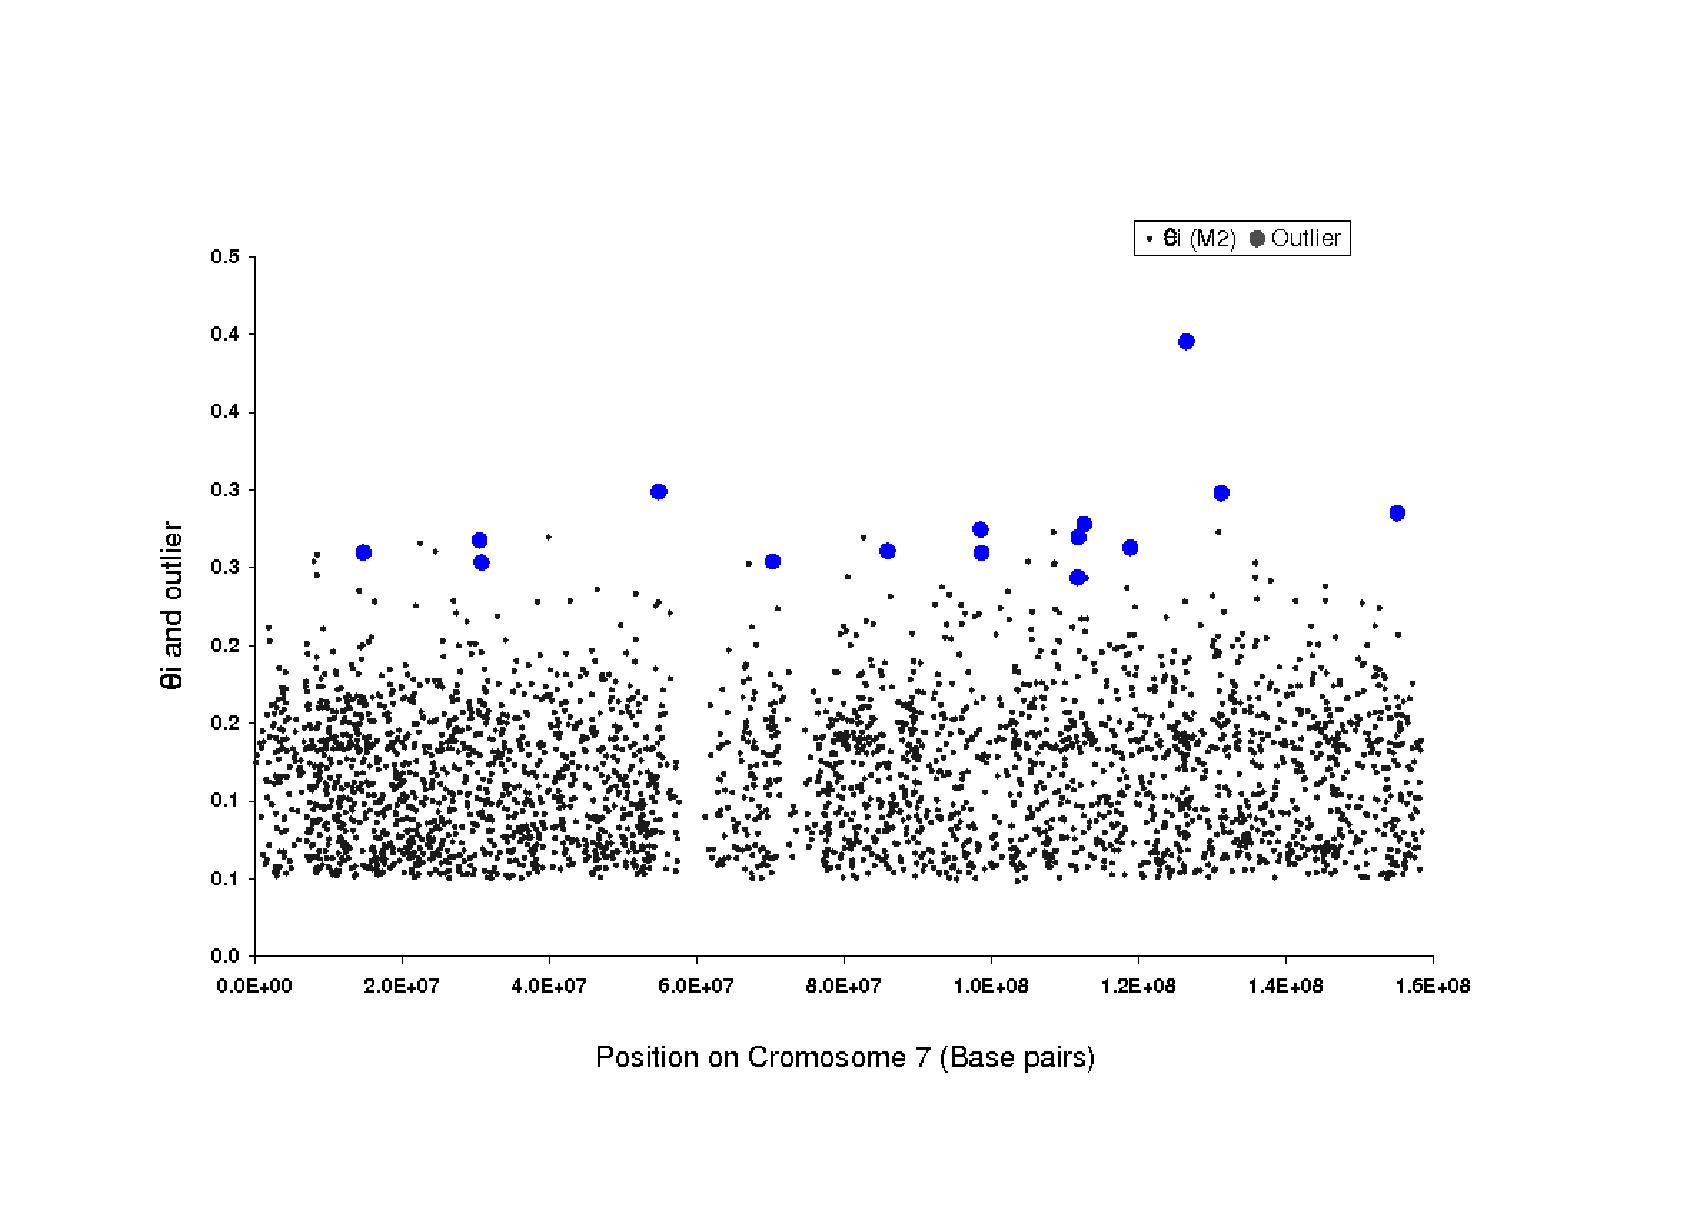
\includegraphics{outlier.eps}}
\end{center}
\caption{Single-locus estimates of $F_{ST}$ along chromosome 7 in the
  HapMap data set. Blue dots denote outliers. Adjacent SNPs in this
  sample are separated, on average, by about
  52kb. (from~\cite{Guo-etal-2009})}\label{fig:low-res-SNP}
\end{figure}

\begin{figure}
\begin{center}
\resizebox{!}{0.8\textheight}{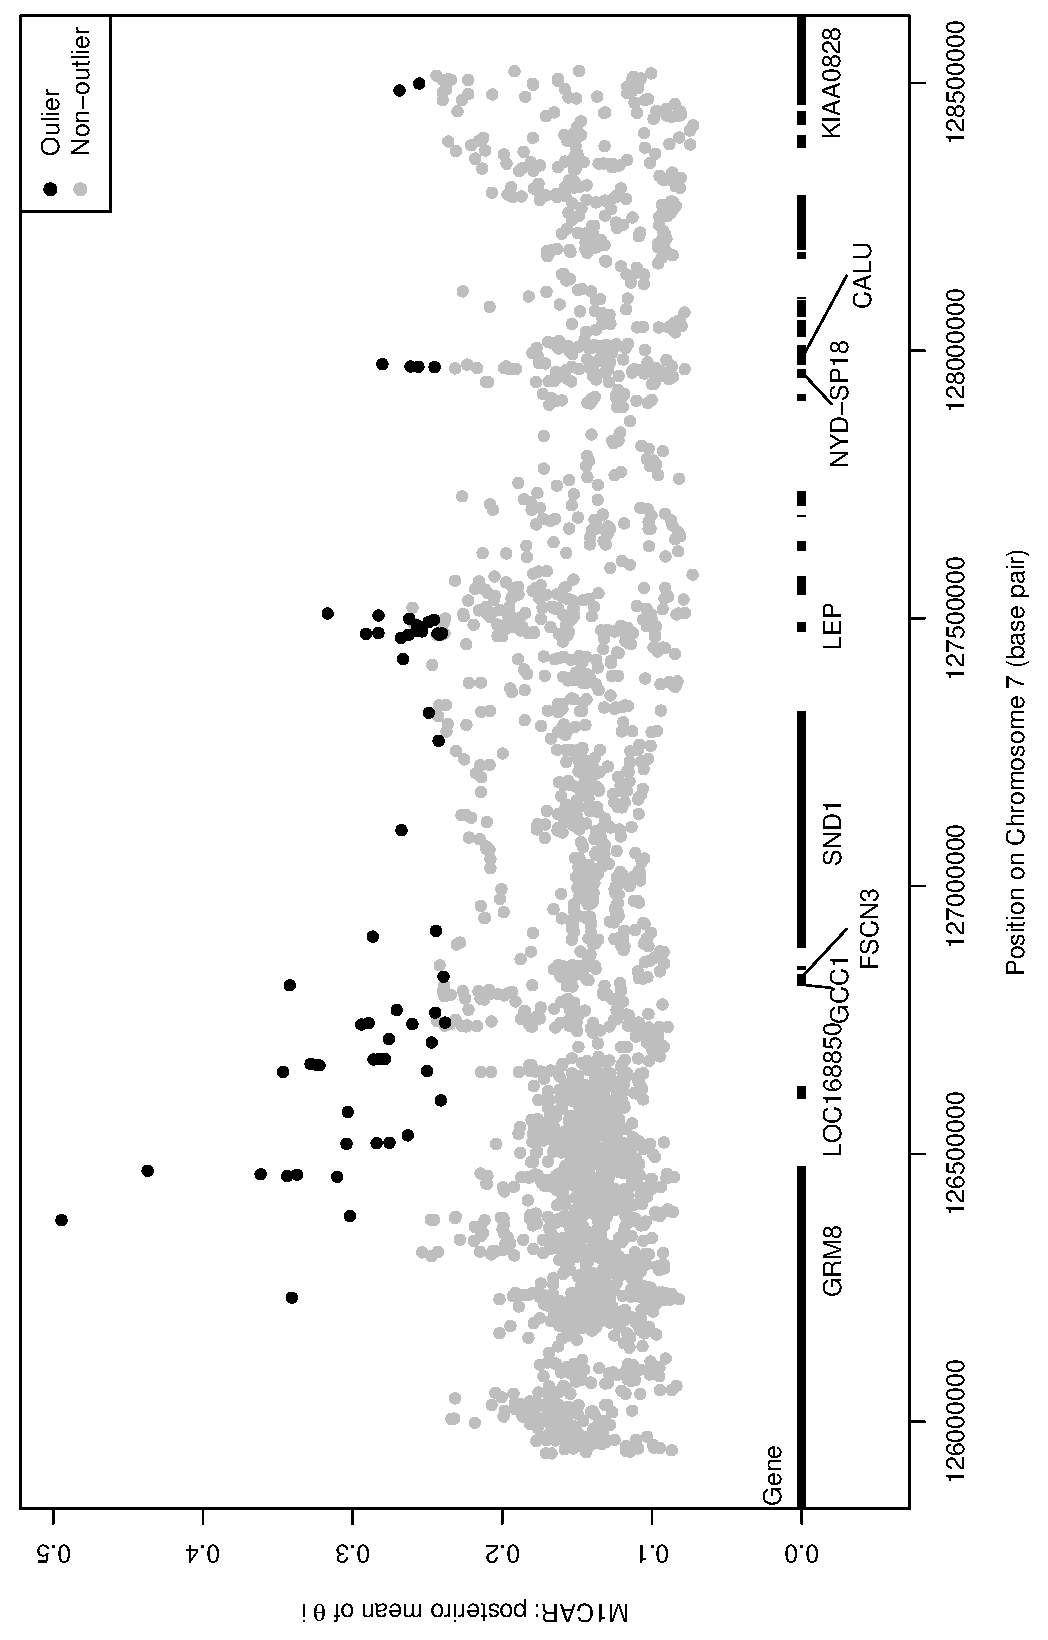
\includegraphics{outlier-high.eps}}
\end{center}
\caption{Single-locus estimates of $F_{ST}$ along a portion of
  chromosome 7 in the HapMap data set. Black dots denote
  outliers. Solid bars refert to previously identified genes. Adjacent
  SNPs in this sample are separated, on average, by about
  1kb. (from~\cite{Guo-etal-2009})}\label{fig:high-res-SNP}
\end{figure}

\section*{Tajima's $D$, Fu's $F_S$, Fay and Wu's $H$, and Zeng et al.'s $E$}

So far we've been comparing rates of synonymous and non-synonymous
substitution to detect the effects of natural selection on molecular
polymorphisms. Tajima~\cite{Tajima89} proposed a method that builds on
the foundation of the neutral theory of molecular evolution in a
different way. I've already mentioned the infinite alleles model of
mutation several times. When thinking about DNA sequences a closely
related approximation is to imagine that every time a mutation occurs,
it occurs at a different site.\footnote{Of course, we know this isn't
  true. Multiple substitutions {\it can\/} occur at any site. That's
  why the percent difference between two sequences isn't equal to the
  number of substitutions that have happened at any particular
  site. We're simply assuming that the sequences we're comparing are
  closely enough related that nearly all mutations have occurred at
  different positions.} If we do that, we have an {\it infinite
  sites\/} model of mutation.\index{mutation!infinite sites model}

\subsection*{Tajima's $D$}\index{Tajima's $D$}

When dealing with nucleotide sequences in a population context there
are two statistics of potential interest:

\begin{itemize}

\item The {\it number\/} of nucleotide positions at which a
  polymorphism is found or, equivalently, the number of segregating
  sites, $k$.\index{segregating sites}

\item The average per nucleotide diversity, $\pi$, where $\pi$ is
  estimated as\index{nucleotide diversity}
\[
\pi = \sum x_ix_j\delta_{ij}/N \quad .
\]
In this expression, $x_i$ is the frequency of the $i$th haplotype,
$\delta_{ij}$ is the number of nucleotide sequence differences between
haplotypes $i$ and $j$, and $N$ is the total length of the
sequence.\footnote{I lied, but you must be getting used to that by
  now. This isn't quite the way you estimate it. To get an unbiased
  estimate of pi, you have to multiply this equation by $n/(n-1)$,
  where $n$ is the number of haplotypes in your sample. And, of
  course, if you're Bayesian you'll be even a little more
  careful. You'll estimate $x_i$ using an appropriate prior on
  haplotype frequencies and you'll estimate the probability that
  haplotypes $i$ and $j$ are different at a randomly chosen position
  given the observed number of differences and the sequence
  length. That probability will be close to $\delta_{ij}/N$, but it
  won't be identical.}

\end{itemize}

The quantity $4N_e\mu$ comes up a lot in mathematical analyses of
molecular evolution. Population geneticists, being a lazy bunch, get
tired of writing that down all the time, so they invented the
parameter $\theta = 4N_e\mu$ to save themselves a little
time.\footnote{This is {\it not\/} the same $\theta$ we encountered
  when discussing $F$-statistics. Weir and Cockerham's $\theta$ is a
  different beast. I know it's confusing, but that's the way it
  is. When reading a paper, the context should make it clear which
  conception of $\theta$ is being used. Another thing to be careful of
  is that sometimes authors think of $\theta$ in terms of a haploid
  population. When they do, it's $2N_e\mu$. Usually the context makes
  it clear which definition is being used, but you have to remember to
  pay attention to be sure.} Under the infinite-sites model of DNA
sequence evolution, it can be shown that
\begin{eqnarray*}
\E(\pi) &=& \theta \\
\E(k) &=& \theta\sum_i^{n-1} \frac{1}{i} \quad ,
\end{eqnarray*}
where $n$ is the number of haplotypes in your sample.\footnote{The
  ``E'' refers to expectation. It is the average value of a random
  variable. $\mbox{E}(\pi)$ is read as ``the expectation of $\pi$>}
This suggests that there are two ways to estimate $\theta$, namely
\begin{eqnarray*}
\hat \theta_\pi &=& \hat \pi \\
\hat \theta_k   &=& \frac{k}{\sum_i^{n-1}\frac{1}{i}} \quad ,
\end{eqnarray*}
where $\hat\pi$ is the average heterozygosity at nucleotide sites in
our sample and $k$ is the observed number of segregating sites in our
sample.\footnote{If your memory is really good, you may recognize that
  those estimates are method of moments estimates, i.e., parameter
  estimates obtained by equating sample statistics with their expected
  values.} If the nucleotide sequence variation among our haplotypes
is neutral and the population from which we sampled is in equilibrium
with respect to drift and mutation, then $\hat\theta_\pi$ and
$\hat\theta_k$ should be statistically indistinguishable from one
another. In other words, 
\[
\hat D = \hat\theta_\pi - \hat\theta_k 
\]
should be indistinguishable from zero. If it is either negative or
positive, we can infer that there's some departure from the
assumptions of neutrality and/or equilibrium. Thus, $\hat D$ can be
used as a test statistic to assess whether the data are consistent
with the population being at a neutral mutation-drift
equilibrium. Consider the value of $D$ under following
scenarios:\index{Tajima's $D$!interpretation}

\begin{description}

\item[Neutral variation] If the variation is neutral and the
  population is at a drift-mutation equilibrium, then $\hat D$ will be
  statistically indistinguishable from zero.

\item[Overdominant selection] Overdominance will allow alleles
  beloning to the different classes to become quite divergent from one
  another. $\delta_{ij}$ within each class will be small, but
  $\delta_{ij}$ between classes will be large and both classes will be
  in intermediate frequency, leading to large values of
  $\theta_\pi$. There won't be a similar tendency for the {\it
  number\/} of segregating sites to increase, so $\theta_k$ will be
  relatively unaffected. As a result, $\hat D$ will be positive.

\item[Population bottleneck] If the population has recently undergone
  a bottleneck, then $\pi$ will be little affected unless the
  bottleneck was prolonged and severe.\footnote{Why? Because most of
    the heterozygosity is due to alleles of moderate to high
    frequency, and those are not the ones likely to be lost in a
    bottleneck. See the Appendix\ref{sect:appendix} for more details.}
  $k$, however, may be substantially reduced. Thus, $\hat D$ should be
  positive.

\item[Purifying selection] If there is purifying selection, mutations
  will occur and accumulate at silent sites, but they aren't likely
  ever to become very common. Thus, there are likely to be lots of
  segregating sites, but not much heterozygosity, meaning that
  $\hat\theta_k$ will be large, $\hat\theta_\pi$ will be small, and
  $\hat D$ will be negative.

\item[Population expansion] Similarly, if the population has recently
  begun to expand, mutations that occur are unlikely to be lost,
  increasing $\hat\theta_k$, but it will take a long time before they
  contribute to heterozygosity, $\hat\theta_\pi$. Thus, $\hat D$ will
  be negative.

\end{description}

In short, $\hat D$ provides a different avenue for insight into the
evolutionary history of a particular nucleotide sequence. But
interpreting it can be a little tricky. 

\begin{description}

\item[$\hat D = 0$:] We have no evidence for changes in population
  size or for any particular pattern of selection at the
  locus.\footnote{Please remember that the failure to detect a difference
    from 0 could mean that your sample size is too small to detect an
    important effect. If you can't detect a difference, you should try
    to assess what values of $D$ are consistent with your data and be
    appropriately circumspect in your conclusions.}

\item[$\hat D < 0$:] The population size may be increasing or we may
  have evidence for purifying selection at this locus.

\item[$\hat D > 0$:] The population may have suffered a recent
  bottleneck (or be decreaing) or we may have evidence for
  overdominant selection at this locus.

\end{description}

\noindent If we have data available for more than one locus, we may be
able to distinguish changes in population size from selection at any
particular locus. After all, all loci will experience the same
demographic effects, but we might expect selection to act differently
at different loci, especially if we choose to analyze loci with
different physiological function.

A quick search in Google Scholar reveals that the paper in which
Tajima described this approach~\cite{Tajima89} has been cited over
5300 times. Clearly it has been widely used for interpreting patterns
of nucleotide sequence variation. Although it is a very useful
statistic, Zeng et al.~\cite{Zeng-etal-2006} point out that there are
important aspects of the data that Tajima's $D$ does not consider. As
a result, it may be less powerful, i.e., less able to detect
departures from neutrality, than some alternatives.

\subsection*{Fu's $F_S$}\index{Fu's $F_S$}

Fu~\cite{Fu-1997} proposes a different statistic based on the infinite
sites model of mutation. He suggests estimating the probability of
observing a random sample with a number of alleles equal to or smaller
than the observed value under given the observed level of diversity
and the assumption that all of the alleles are selectively neutral. If
we call this probability $\hat S$, then
\[
F_S = \ln\left(\frac{\hat S}{1 - \hat S}\right) \quad .
\]
A negative value of $F_S$ is evidence for an excess number of alleles,
as would be expected from a recent population expansion or from
genetic hitchhiking. A positive value of $F_S$ is evidence for an
deficiency of alleles, as would be expect from a recent population
bottleneck or from overdominant selection. Fu's simulations suggest
that $F_S$ is a more sensitive indicator of population expansion and
genetic hitchhiking than Tajima�s $D$. Those simulations also suggest
that the conventional P-value of 0.05 corresponds to a P-value from
the coalescent simulation of 0.02. In other words, $F_S$ should be
regarded as significant if $P < 0.02$.

\subsection*{Fay and Wu's $H$}\index{Fay and Wu's $H$}

Let $\xi_i$ be the number of sites at which a sequence occurring $i$
times in the sample differs from the sequence of the most recent
common ancestor for all the sequences. Fu~\cite{Fu-1995} showed that
\[
\mbox{E}(\xi_i) = \frac{\theta}{i} \quad .
\]
Remember that $i$ is the number of times this haplotype occurs in the
sample. Using this result, we can rewrite $\hat\theta_\pi$ and
$\hat\theta_k$ as
\begin{eqnarray*}
\hat\theta_\pi &=& {n \choose 2}^{-1}\sum_{i=1}^{n-1}i(n-i)\hat\xi_i \\
\hat\theta_k  &=& \frac{1}{a_n}\sum_{i=1}^{n-1}\hat\xi_i
\end{eqnarray*}
There are also at least two other statistics that could be used to
estimate $\theta$ from these data:
\begin{eqnarray*}
\theta_H &=& {n \choose 2}^{-1}\sum_{i=1}^{n-1}i^2\hat\xi_i \\
\theta_L &=& \frac{1}{n-1}\sum_{i=1}^{n-1}i\hat\xi_i \quad .
\end{eqnarray*}
Notice that to estimate $\theta_H$ or $\theta_L$, you'll
need information on the sequence of an ancestral haplotype. To get
this you'll need an outgroup. As we've already seen, we can get
estimates of $\theta_\pi$ and $\theta_k$ without an outgroup.

Fay and Wu~\cite{Fay-Wu-2000} suggest using the statistic
\[
H = \hat\theta_\pi - \theta_H 
\]
to detect departures from neutrality. So what's the difference between
Fay and Wu's $H$ and Tajima's $D$?  Well, notice that there's an $i^2$
term in $\theta_H$. The largest contributions to this estimate of
$\theta$ are coming from alleles in relatively high frequency, i.e.,
those with lots of copies in our sample. In contrast,
intermediate-frequency alleles contribute most to estiamtes of
$\theta_\pi$. Thus, $H$ measures departures from neutrality that are
reflected in the difference between high-frequency and
intermediate-frequency alleles. In contrast, $D$ measures departures
from neutrality that are reflected in the difference between
low-frequency and intermediate frequency alleles.  Thus, while $D$ is
sensitive to population expansion (because the number of segregating
sites responds more rapidly to changes in population size than the
nucleotide heterozygosity), $H$ will not be. As a result, combining
both tests may allow you to distinguish populaion expansion from
purifying selection.

\subsection*{Zeng et al.'s $E$}\index{Zeng et al.'s $E$}

So if we can use $D$ to compare estimates of $\theta$ from
intermediate- and low-frequency variants and $H$ to compare estimates
from intermediate- and high-frequency variatnts, what about comparing
estimates from high-frequency and low-frequency variants? Funny you
should ask, Zeng et al.~\cite{Zeng-etal-2006} suggest looking at
\[
E = \theta_L - \theta_k \quad . 
\]
$E$ doesn't put quite as much weight on high frequency variants as
$H$,\footnote{Because it has an $i$ rather than an $i^2$ in its
  formula} but it still provides a useful contrast between estimates
of $\theta$ dertived from high-frequency variants and low-frequency
variants. For example, suppose a new favorable mutation occurs and
sweeps to fixation. All alleles other than those carrying the new
allele will be eliminated from the population. Once the new variant is
established, neutral variaton will begin to accumulate. The return to
neutral expectations after such an event, however, happens much more
rapidly in low frequency variants than in high-frequency ones. Thus, a
negative $E$ may provide evicence of a recent selective sweep at the
locus being studied. For similar reasons, it will be a sensitive
indicator of recent population expansion.

\section*{Appendix}\label{sect:appendix}

I noted earlier that $\pi$ will be little affected by a population
bottleneck unless it is prolonged and severe. Here's one way of
thinking about it that might make that counterintuitive assertion a
little clearer.

Remember that $\pi$ is defined as $\pi = \sum
x_ix_j\delta_{ij}/N$. Unless one haplotype in the population happens
to be very divergent from all other haplotypes in the population, the
magnitude of $\pi$ will be approximately equal to the average
difference between any two nucleotide sequences times the probability
that two randomly chosen sequences represent different
haplotypes. Thus, we can treat haplotypes as alleles and ask what
happens to heterozygosity as a result of a bottleneck. Here we recall
the relationship between identity by descent and drift, and we pretend
that homozygosity is the same thing as identity by descent. If we do,
then the heterozygosity after a bottleneck is
\[
H_t = \left(1 - \frac{1}{2N_e}\right)^tH_{0} \quad.
\]
So consider a {\it really\/} extreme case: a population reduced to one
male and one female for 5 generations. $N_e=2$, so $H_5 \approx
0.24H_0$, so the population would retain roughly 24\% of its original
diversity even after such a bottleneck. Suppose it were less severe,
say, five males and five females for 10 generations, then $N_e=10$ and
$H_{10} \approx 0.6$.



\bibliography{popgen}
\bibliographystyle{plain}

\ccLicense

\end{document}


